\documentclass[aspectratio=169]{beamer}

\usetheme{metropolis}
\usepackage{appendixnumberbeamer}

\usepackage{amsmath}
\usepackage{amssymb}
\usepackage{mathtools}
\usepackage{booktabs}
\usepackage{colortbl}
\usepackage{tikz}
\usepackage{pgfplots}
\pgfplotsset{compat=1.18}
\usepackage{graphicx}
\usepackage{subcaption}
\usepackage{algorithm}
\usepackage{algorithmic}
\usepackage[backend=bibtex,style=authoryear,natbib,maxcitenames=2]{biblatex}
\addbibresource{../iclr2026_conference.bib}

% Path to figures (relative from Slides/)
\graphicspath{{../Figures/}}

% Custom colors
\definecolor{mkgreen}{RGB}{0,128,80}
\definecolor{nmblue}{RGB}{50,100,180}
\definecolor{alertorange}{RGB}{220,100,30}

\setbeamercolor{block title}{bg=mkgreen!20, fg=black}
\setbeamercolor{block body}{bg=mkgreen!5}

\title{Markovian Transformers for\\Informative Language Modeling}
\author{Scott W.\ Viteri \and Max Lamparth \and Peter Chatain \and Clark Barrett}
\institute{Department of Computer Science, Stanford University}
\date{ICLR 2026}

\begin{document}

% ============================================================
\begin{frame}[plain]
\maketitle
\end{frame}

% ============================================================
\begin{frame}{The Problem: Chain-of-Thought is Not Faithful}

\begin{columns}[T]
\column{0.55\textwidth}
\textbf{Chain-of-Thought (CoT) prompting} lets LMs ``show their work''
\citep{wei2022chain, nye2022show}

\bigskip
But CoTs can be \alert{unfaithful}:
\begin{itemize}
    \item Spurious biases remain hidden \citep{turpin2023language}
    \item Altering the CoT may not change the answer \citep{lanham2023measuring}
    \item The model can \textbf{bypass} the CoT entirely
\end{itemize}

\column{0.42\textwidth}
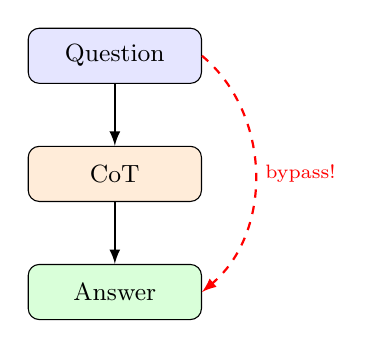
\begin{tikzpicture}[
    box/.style={rectangle, draw, rounded corners, minimum width=2.2cm,
                minimum height=0.7cm, font=\small},
    arrow/.style={->, thick, >=latex}
]
\node[box, fill=blue!10] (Q) at (0,3) {Question};
\node[box, fill=orange!15] (C) at (0,1.5) {CoT};
\node[box, fill=green!15] (A) at (0,0) {Answer};
\draw[arrow] (Q) -- (C);
\draw[arrow] (C) -- (A);
\draw[arrow, red, dashed, thick] (Q.east) to[bend left=50]
    node[right, font=\scriptsize, text=red]{bypass!} (A.east);
\end{tikzpicture}

\vspace{0.3cm}
{\small\color{red} Standard models can still ``see'' the question when generating the answer.}
\end{columns}
\end{frame}

% ============================================================
\begin{frame}{Our Approach: The Markovian Bottleneck}

\textbf{Key insight}: remove the architectural escape hatch.

\begin{center}
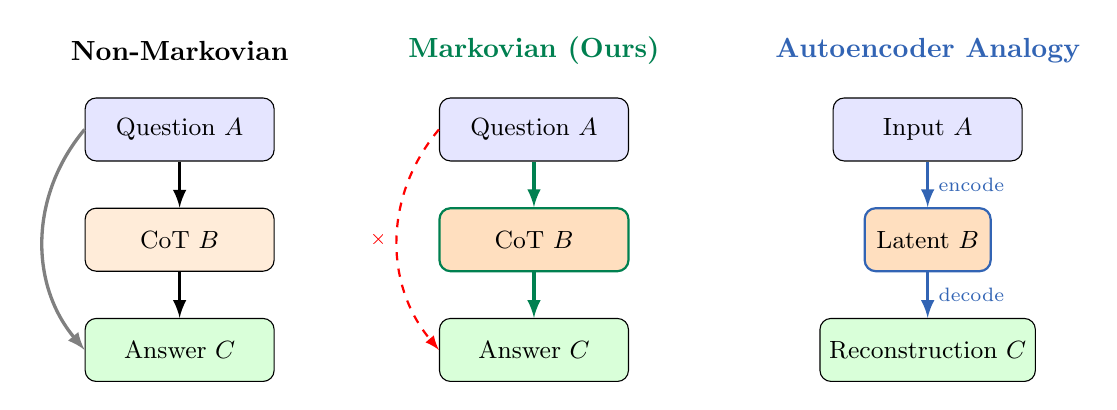
\begin{tikzpicture}[
    box/.style={rectangle, draw, rounded corners, minimum width=2.4cm,
                minimum height=0.8cm, font=\small},
    arrow/.style={->, very thick, >=latex}
]
% Non-Markovian
\node[font=\bfseries] at (-4.5,3.2) {Non-Markovian};
\node[box, fill=blue!10] (Q1) at (-4.5,2.2) {Question $A$};
\node[box, fill=orange!15] (C1) at (-4.5,0.8) {CoT $B$};
\node[box, fill=green!15] (A1) at (-4.5,-0.6) {Answer $C$};
\draw[arrow] (Q1) -- (C1);
\draw[arrow] (C1) -- (A1);
\draw[arrow, gray] (Q1.west) to[bend right=40] (A1.west);

% Markovian
\node[font=\bfseries, text=mkgreen] at (0,3.2) {Markovian (Ours)};
\node[box, fill=blue!10] (Q2) at (0,2.2) {Question $A$};
\node[box, fill=orange!25, thick, draw=mkgreen] (C2) at (0,0.8) {CoT $B$};
\node[box, fill=green!15] (A2) at (0,-0.6) {Answer $C$};
\draw[arrow, mkgreen] (Q2) -- (C2);
\draw[arrow, mkgreen] (C2) -- (A2);
\draw[arrow, red, dashed, thick] (Q2.west) to[bend right=40]
    node[left, font=\scriptsize, text=red]{\texttimes} (A2.west);

% Autoencoder
\node[font=\bfseries, text=nmblue] at (5,3.2) {Autoencoder Analogy};
\node[box, fill=blue!10] (E) at (5,2.2) {Input $A$};
\node[box, fill=orange!25, thick, draw=nmblue,
      minimum width=1.6cm] (L) at (5,0.8) {Latent $B$};
\node[box, fill=green!15] (D) at (5,-0.6) {Reconstruction $C$};
\draw[arrow, nmblue] (E) -- node[right, font=\scriptsize]{encode} (L);
\draw[arrow, nmblue] (L) -- node[right, font=\scriptsize]{decode} (D);
\end{tikzpicture}
\end{center}

\vspace{0.1cm}
The CoT becomes a \textbf{bandwidth bottleneck}: all information from $A$ to $C$ must flow through $B$.
\end{frame}

% ============================================================
\begin{frame}{Formal Framework: Markovian Language Model}

\begin{block}{Definition}
\scriptsize
A \textbf{Markovian LM} is a tuple $M = (\mathcal{O}, \mathcal{S}, \pi, u, s_1)$:
\begin{itemize}
    \itemsep 0.1em
    \item $\mathcal{O}$: observations \quad (questions, answers)
    \item $\mathcal{S}$: states \quad (CoT reasoning text)
    \item $\pi: \mathcal{S} \to \Delta(\mathcal{O})$: policy --- predicts observations \textbf{from state alone}
    \item $u: \mathcal{O} \times \mathcal{S} \to \Delta(\mathcal{S})$: state update --- produces CoT from question + prior state
    \item $s_1 \in \mathcal{S}$: initial state
\end{itemize}
\end{block}

\vspace{-0.45cm}
\begin{center}
\resizebox{0.5\textwidth}{!}{%
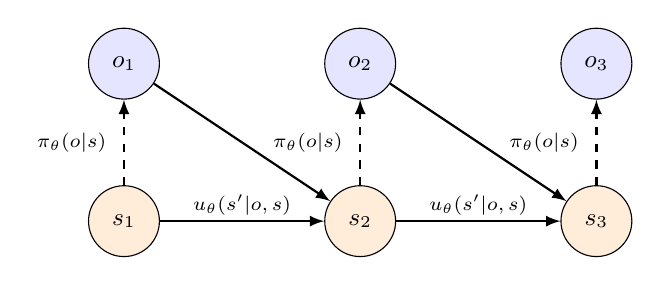
\begin{tikzpicture}[
    circ/.style={circle, draw, minimum size=0.9cm, font=\small},
    arrow/.style={->, thick, >=latex}
]
\node[circ, fill=blue!10] (o1) at (0,1.5) {$o_1$};
\node[circ, fill=blue!10] (o2) at (3,1.5) {$o_2$};
\node[circ, fill=blue!10] (o3) at (6,1.5) {$o_3$};
\node[circ, fill=orange!15] (s1) at (0,-0.5) {$s_1$};
\node[circ, fill=orange!15] (s2) at (3,-0.5) {$s_2$};
\node[circ, fill=orange!15] (s3) at (6,-0.5) {$s_3$};

\draw[arrow] (o1) -- (s2);
\draw[arrow] (s1) -- (s2);
\draw[arrow] (o2) -- (s3);
\draw[arrow] (s2) -- (s3);
\draw[arrow, dashed] (s1) -- (o1);
\draw[arrow, dashed] (s2) -- (o2);
\draw[arrow, dashed] (s3) -- (o3);

\node[font=\scriptsize] at (1.5,-0.3) {$u_\theta(s'|o,s)$};
\node[font=\scriptsize] at (4.5,-0.3) {$u_\theta(s'|o,s)$};
\node[font=\scriptsize, left] at (-0.1,0.5) {$\pi_\theta(o|s)$};
\node[font=\scriptsize, left] at (2.9,0.5) {$\pi_\theta(o|s)$};
\node[font=\scriptsize, left] at (5.9,0.5) {$\pi_\theta(o|s)$};
\end{tikzpicture}
}
\end{center}
\end{frame}

% ============================================================
\begin{frame}{Informativeness Objective \& Reward}

\textbf{Reward}: how much better is the trained CoT than the frozen baseline?
\[
R_\theta = \underbrace{\ln \pi_\theta(\text{ans} \mid \text{CoT})}_{\text{trained actor on trained CoT}}
          \;-\; \underbrace{\ln \pi'(\text{ans} \mid \text{CoT}')}_{\text{frozen baseline on baseline CoT}}
\]

\textbf{Objective}: maximize expected informativeness
\[
J(\theta) = \mathbb{E}_{\tau \sim P, u_\theta, u'}[R_\theta(\tau)]
\]

\begin{block}{Coding-Theoretic Interpretation}
\begin{itemize}
    \item $-\log \pi_\theta(C \mid B)$: coding cost of the answer given the CoT
    \item $-\log u'(B \mid A)$: coding cost of the CoT under the prior
    \item Training searches for short states $B$ that make both legs $A \to B \to C$ efficient
\end{itemize}
\end{block}
\end{frame}

% ============================================================
\begin{frame}{Training: GRPO-Style Policy Gradient}

\textbf{Key innovation}: the reward $R_\theta$ depends on $\theta$, so we get two gradient terms:
\[
\nabla_\theta\, \mathbb{E}[R_\theta(\tau)]
= \mathbb{E}\!\Big[\;\;\underbrace{R_\theta \cdot \nabla_\theta \ln P_\theta(\tau)}_{\text{policy gradient}}
  \;\;\;+\;\;\; \underbrace{\nabla_\theta R_\theta(\tau)}_{\text{actor-reward gradient}}\Big]
\]
\vspace{-0.35cm}

\textbf{Loss function} (three components):
\[
\mathcal{L} = \underbrace{\mathcal{L}_{\text{PG}}}_{\text{REINFORCE}} + \underbrace{\mathcal{L}_{\text{AR}}}_{\text{direct reward}} + \underbrace{\mathcal{L}_{\text{KL}}}_{\text{regularization}}
\]
\vspace{-0.25cm}

\begin{itemize}
    \itemsep 0.2em
    \item \textbf{Parallel sampling}: $B$ diverse CoTs per question (GRPO-style)
    \item \textbf{Within-batch standardization}: advantages have zero mean, unit variance
    \item \textbf{KL penalty} ($\beta = 0.1$): discourages steganographic encodings
    \item \textbf{LoRA} (rank 8): stable fine-tuning with frozen base weights
\end{itemize}
\end{frame}

% ============================================================
\begin{frame}{Training Algorithm}

\begin{algorithm}[H]
\caption{Markovian Training (GRPO-Style)}
\small
\begin{algorithmic}[1]
\STATE \textbf{Given}: dataset $P$, actor $(u_\theta, \pi_\theta)$, frozen baseline $(u', \pi')$, batch size $B$
\FOR{each training batch}
  \STATE Sample $(q, a) \sim P$
  \STATE Sample $\text{CoT}_i \sim u_\theta(\cdot \mid q)$ for $i = 1 \ldots B$ \hfill {\color{gray}\textit{parallel sampling}}
  \STATE Sample baseline $\text{CoT}' \sim u'(\cdot \mid q)$ \hfill {\color{gray}\textit{once per batch}}
  \STATE Compute $r_i = \ln \pi_\theta(a \mid \text{CoT}_i)$, \quad $b = \ln \pi'(a \mid \text{CoT}')$
  \STATE Standardize: $A_i = (r_i - b - \mu) / (\sigma + \epsilon)$
  \STATE $\ell_i = \underbrace{-\ln u_\theta(\text{CoT}_i \mid q) \cdot A_i^{\text{detach}}}_{\mathcal{L}_{\text{PG}}} + \underbrace{(-A_i)}_{\mathcal{L}_{\text{AR}}} + \underbrace{\beta_{\text{KL}}\, D_{\text{KL}}}_{\mathcal{L}_{\text{KL}}}$
  \STATE Update $\theta$ with $\frac{1}{B} \sum_i \ell_i$
\ENDFOR
\end{algorithmic}
\end{algorithm}
\end{frame}

% ============================================================
\begin{frame}{Experimental Setup}

\textbf{Two evaluation regimes}:

\begin{columns}[T]
\column{0.48\textwidth}
\textbf{1.\ Question--Answer Tasks}
\begin{itemize}
    \item GSM8K (grade-school math)
    \item MMLU (multitask QA)
    \item SVAMP (math word problems)
    \item ARC-Challenge (science MCQ)
    \item Arithmetic (15-term addition)
\end{itemize}
CoT provides \emph{additional computation}

\column{0.48\textwidth}
\textbf{2.\ Wikipedia Continuation}
\begin{itemize}
    \item 200 tokens context
    \item 50 tokens CoT
    \item 100 tokens target
\end{itemize}
CoT is a \emph{bandwidth bottleneck} that must compress context

\end{columns}

\bigskip
\textbf{Models}: Llama 3.1 8B, Mistral 7B, Qwen3 4B, Phi 3.5

\textbf{Training}: LoRA (rank 8, $\alpha=16$), bfloat16, gradient clipping at 1.0
\end{frame}

% ============================================================
\begin{frame}{Results: QA Task Accuracy}

\begin{columns}[T]
\column{0.5\textwidth}
\begin{table}
\centering
\small
\begin{tabular}{lccc}
\toprule
Dataset & Base & Non-Mkv & Mkv \\
\midrule
GSM8K & 19.6\% & 63.3\% & 57.1\% \\
ARC-Chal & 36.1\% & 78.6\% & 79.9\% \\
Arithmetic & 1.0\% & 97.0\% & 98.0\% \\
MMLU & 21.4\% & 68.7\% & 55.5\% \\
SVAMP & 18.0\% & 43.3\% & 42.3\% \\
\bottomrule
\end{tabular}
\end{table}

\column{0.48\textwidth}
\vspace{0.3cm}
\begin{itemize}
    \item Large absolute gains over base model
    \item Within $\approx$3--4\,pp of Non-Markovian
    \item ARC \& Arithmetic: Markovian \emph{beats} Non-Markovian
    \item All this while the model \textbf{cannot see the question} when answering
\end{itemize}
\end{columns}

\vspace{0.5cm}
\begin{center}
\colorbox{mkgreen!10}{\parbox{0.85\textwidth}{\centering
The Markovian constraint forces informative CoTs with minimal accuracy loss.
}}
\end{center}
\end{frame}

%% ============================================================
%\begin{frame}{Results: Wikipedia Continuation Training}
%
%\begin{figure}
%\centering
%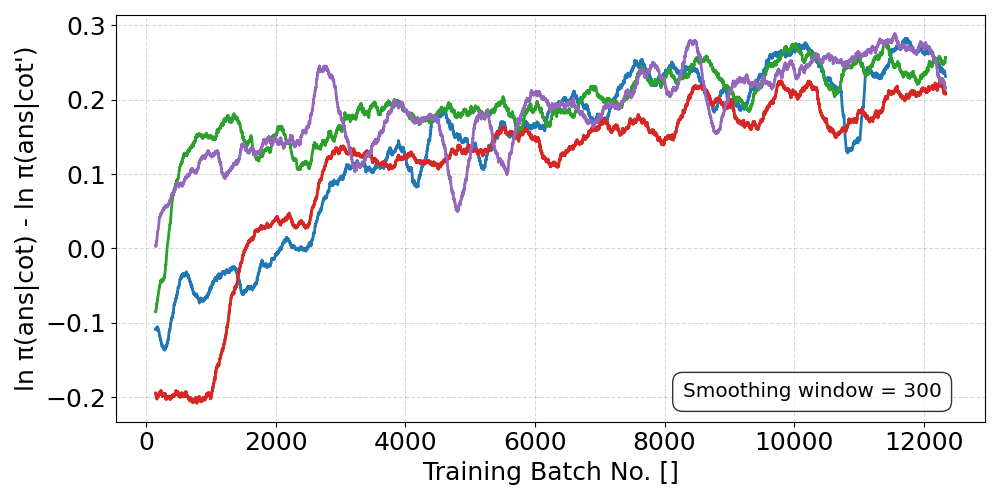
\includegraphics[width=0.65\textwidth]{combined_metrics_wiki_continuation.png}
%\caption{Wikipedia continuation training across 4 random seeds (Llama 8B). Consistent convergence despite high per-batch variance.}
%\end{figure}
%\end{frame}

% ============================================================
\begin{frame}{Perturbation Sensitivity: Is the CoT Load-Bearing?}

\textbf{Experiment}: corrupt the CoT, measure log-probability drop for Markovian vs.\ Non-Markovian.

\begin{table}
\centering
\small
\begin{tabular}{lccccc|c}
\toprule
Severity & CharRep & Delete & DigRep & TruncB & TruncF & Mean \\
\midrule
20\% & +0.46 & +0.46 & +0.02 & +0.25 & $-$0.01 & +0.24 \\
60\% & +1.04 & +1.00 & +0.04 & +0.60 & +0.28 & +0.59 \\
100\% & +1.08 & +1.26 & +0.04 & +1.26 & +1.26 & +0.98 \\
\midrule
\rowcolor{mkgreen!10}
Col.\ Mean & +0.90 & +0.93 & +0.03 & +0.70 & +0.46 & +0.60 \\
\bottomrule
\end{tabular}
\caption*{\small Positive = Markovian more fragile (relies more on intact CoTs). Wikipedia, 1024 examples.}
\end{table}

\vspace{0.2cm}
\begin{center}
Markovian models are \textbf{consistently more sensitive} to CoT corruption $\Rightarrow$ CoT is causally essential.
\end{center}
\end{frame}

% ============================================================
\begin{frame}{QA Perturbation Fragility}

\begin{table}
\centering
\small
\begin{tabular}{lcccccc}
\toprule
\textbf{Dataset} & \textbf{CharRep} & \textbf{Delete} & \textbf{DigRep} & \textbf{TruncB} & \textbf{TruncF} & \textbf{Avg} \\
\midrule
ARC & +0.320 & +0.424 & $-$0.004 & +0.069 & +0.439 & \textbf{+0.250} \\
SVAMP & +0.154 & +0.204 & +0.081 & +0.076 & +0.046 & \textbf{+0.112} \\
GSM8K & +0.059 & +0.069 & $-$0.013 & +0.105 & +0.044 & +0.053 \\
MMLU & +0.056 & +0.124 & +0.004 & +0.038 & $-$0.001 & +0.044 \\
Arithmetic & $-$0.016 & $-$0.003 & $-$0.043 & +0.001 & $-$0.016 & $-$0.015 \\
\midrule
\rowcolor{mkgreen!10}
\textbf{Overall} & \textbf{+0.115} & \textbf{+0.164} & \textbf{+0.005} & \textbf{+0.058} & \textbf{+0.102} & \textbf{+0.089} \\
\bottomrule
\end{tabular}
\caption*{\small Accuracy $\Delta$ (Markovian drop $-$ Non-Markovian drop). Positive = Markovian relies more on CoT.}
\end{table}

ARC shows the clearest Markovian fragility (+25\,pp). Arithmetic is a near-tie because \emph{both} models treat every digit as load-bearing.
\end{frame}

%% ============================================================
%\begin{frame}{Cross-Model Transfer: CoTs Generalize}
%
%\begin{figure}
%\centering
%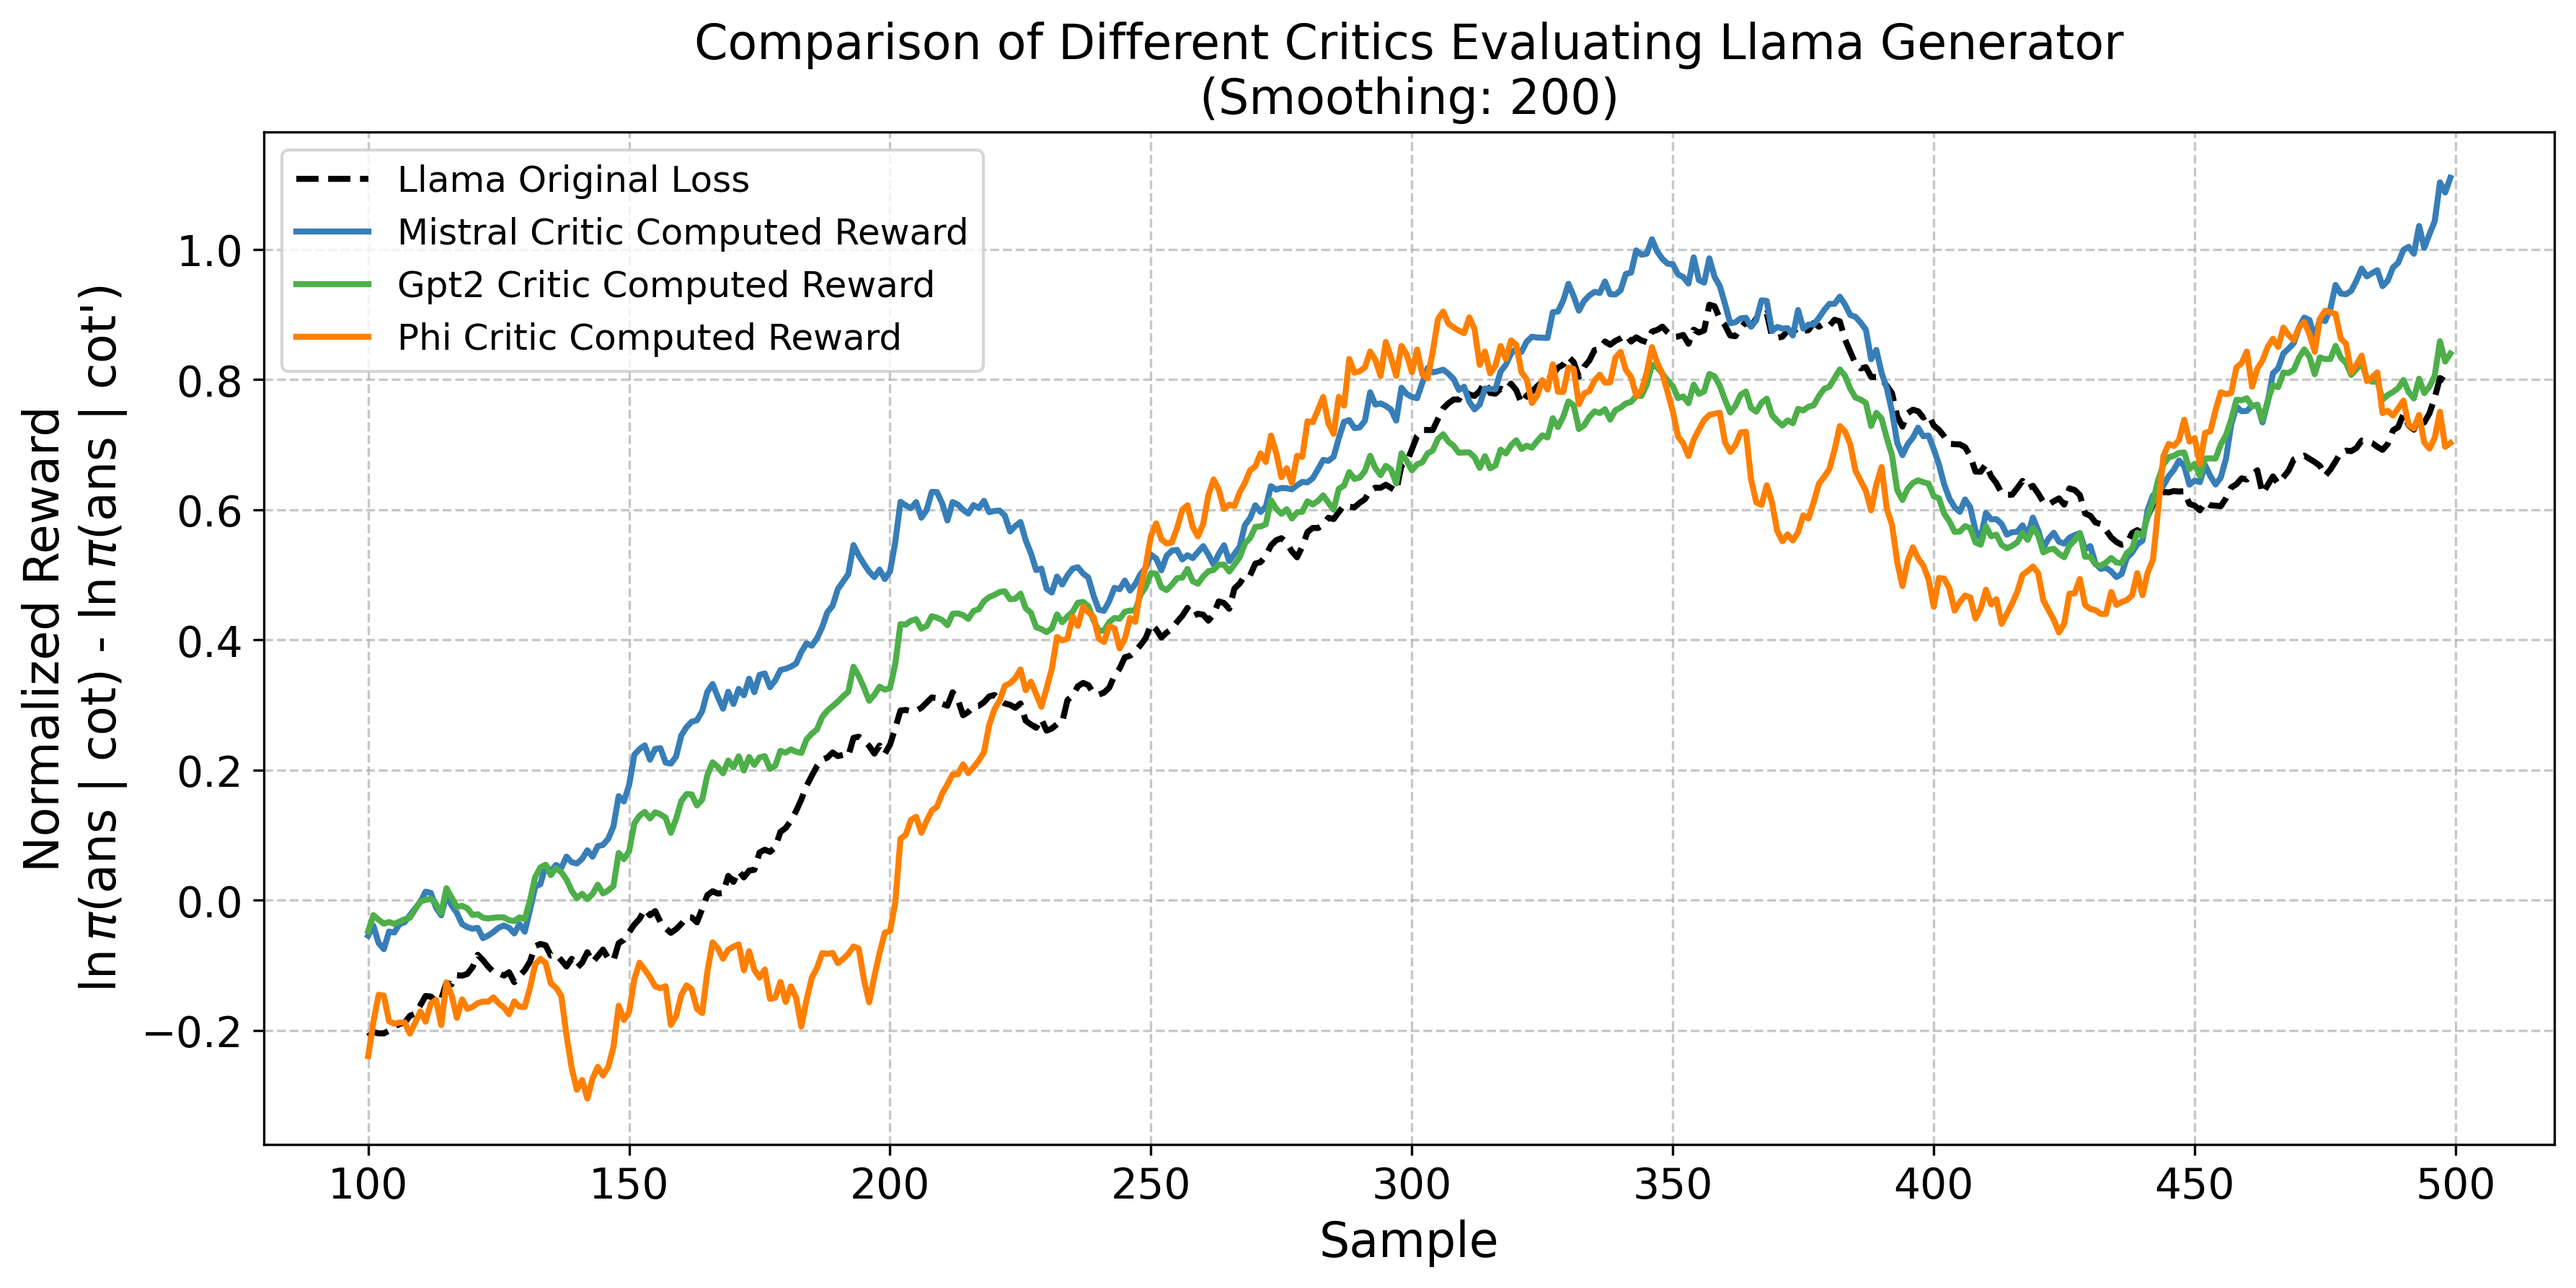
\includegraphics[width=0.6\textwidth]{gsm8k_multiple_critics_comparison.png}
%\caption{Llama 8B's CoTs evaluated by Mistral, GPT-2, and Phi 3.5 on GSM8K. As training progresses, all critics' rewards increase in tandem.}
%\end{figure}
%
%\end{frame}

% ============================================================
\begin{frame}{Cross-Model Transfer: Wikipedia}

\begin{figure}
\centering
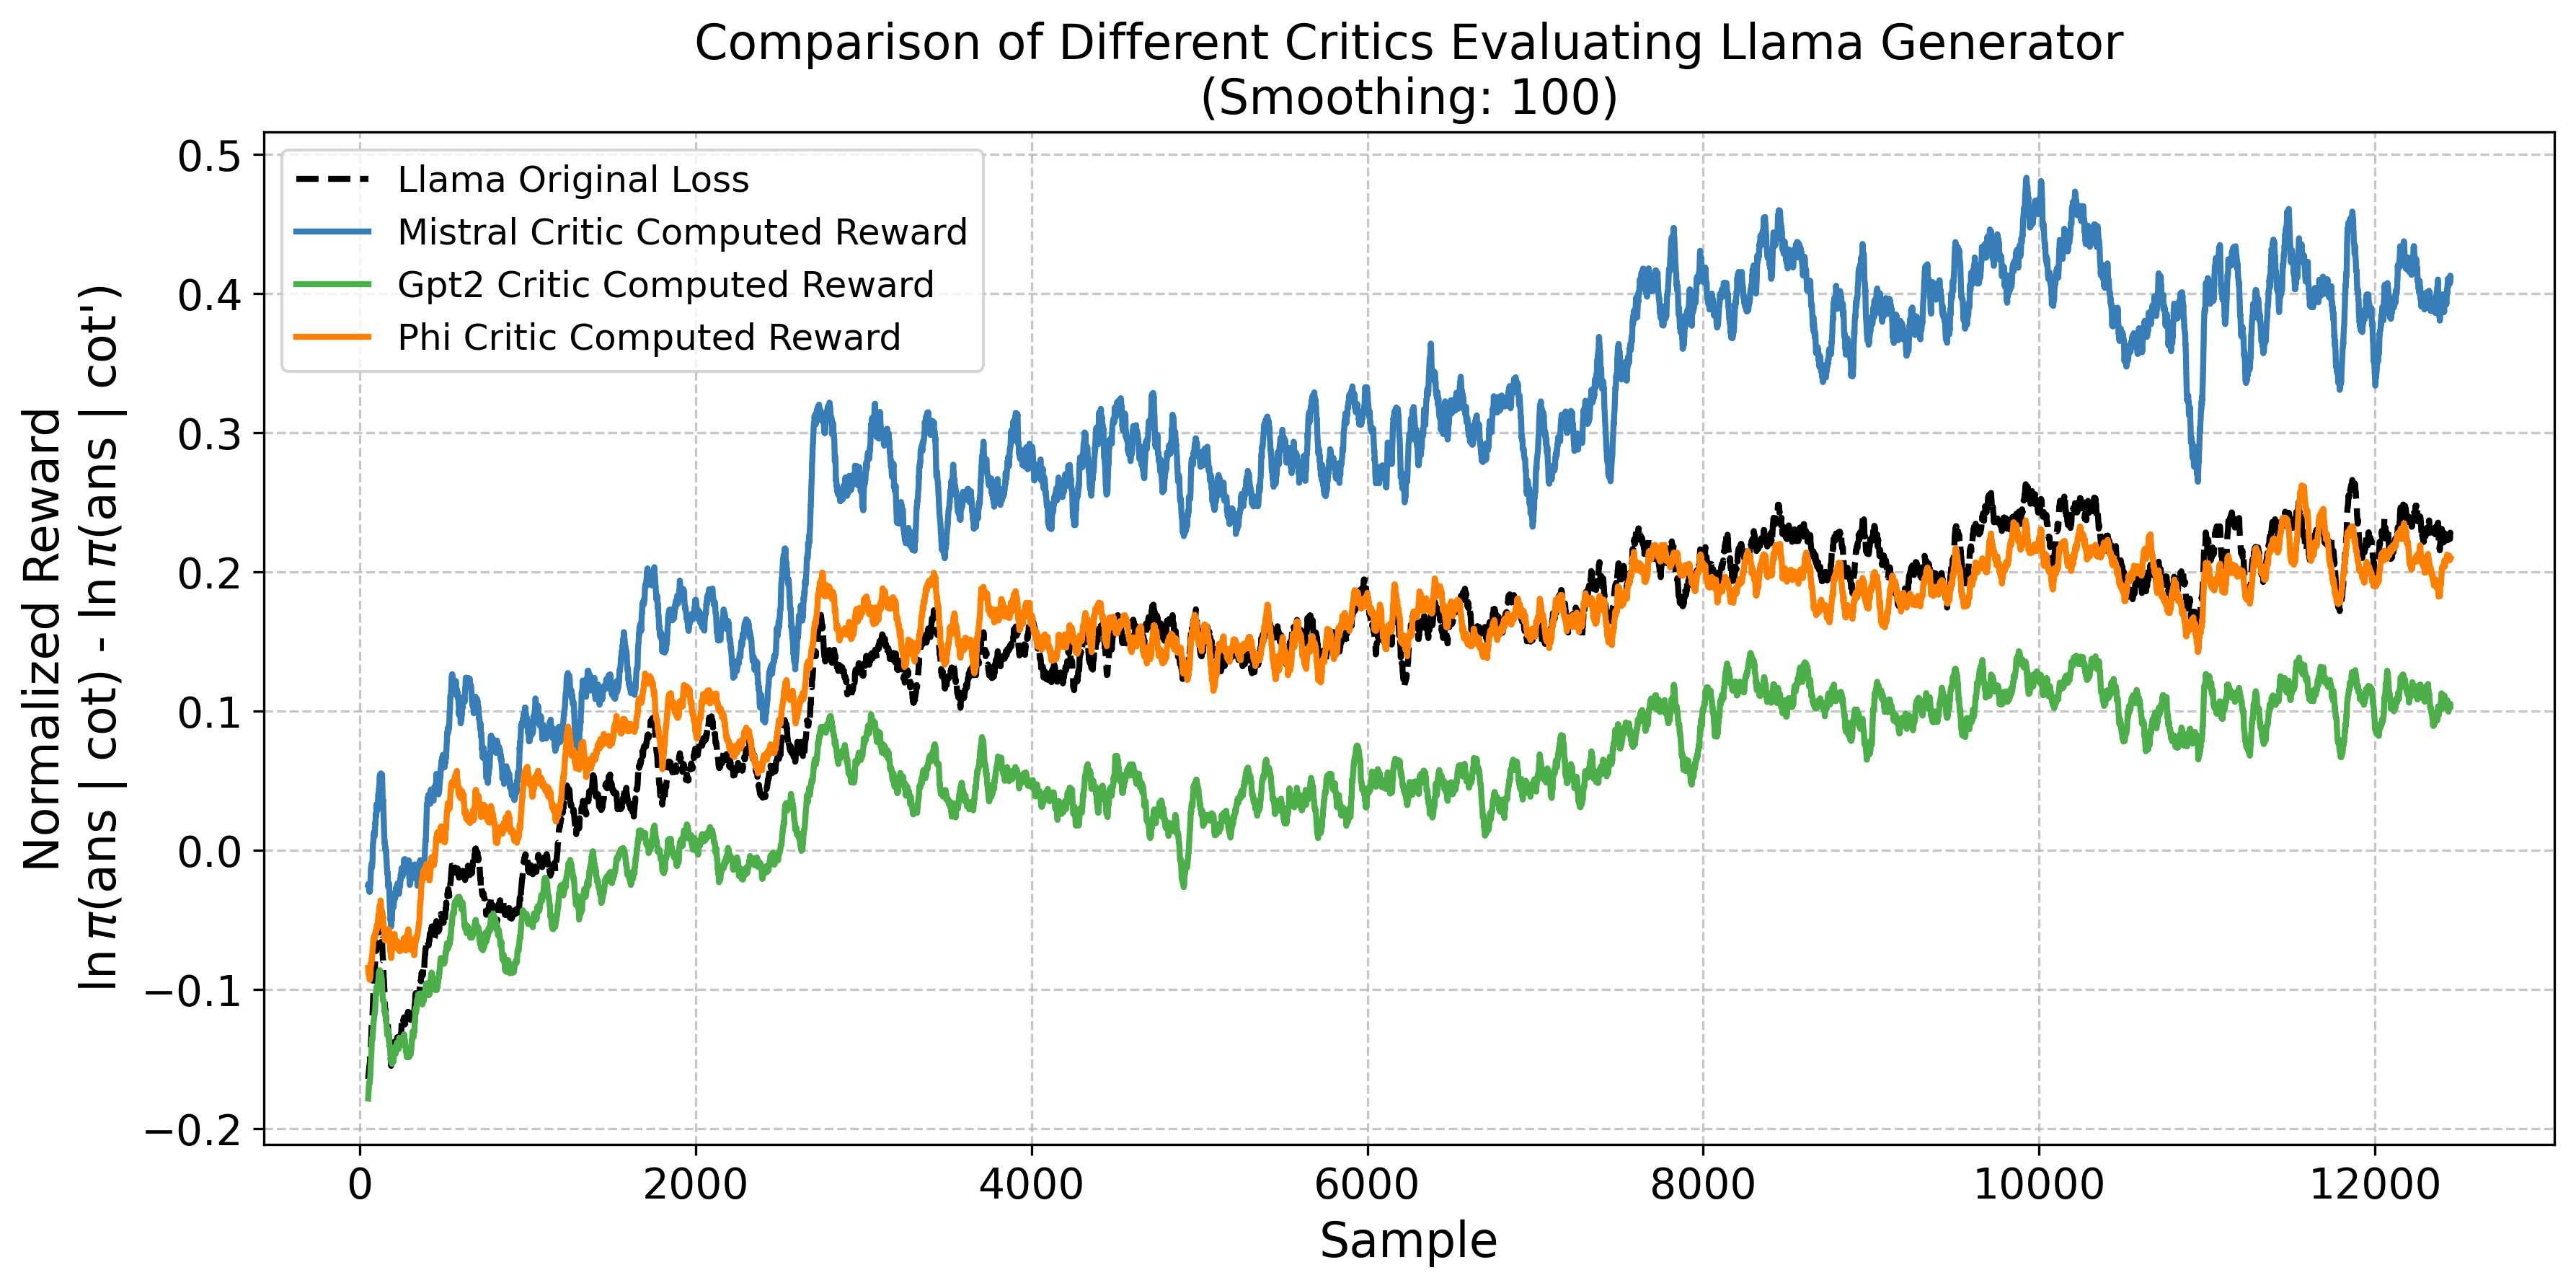
\includegraphics[width=0.8\textwidth]{wiki_multi_critic_comparison.png}
\caption{Llama evaluating Mistral's CoT quality during training on Wikipedia. Correlation between both models' evaluations confirms cross-architecture generalization. Averaged over 6 runs.}
\end{figure}

\vspace{0.1cm}
Transfer even to \textbf{GPT-2} (124M params, cannot decode steganography)\\
$\Rightarrow$ CoTs encode reasoning in \textbf{natural language}, not model-specific artifacts.
\end{frame}

%% ============================================================
%\begin{frame}{Algorithmic Ablations}
%
%\begin{table}
%\centering
%\small
%\begin{tabular}{lccccc}
%\toprule
%\textbf{Dataset} & \textbf{Base} & \textbf{EI} & \textbf{No Rew.\ Grad} & \textbf{Markovian} & \textbf{Non-Mkv} \\
%\midrule
%GSM8K & 19.6\% & 61.6\% & 62.2\% & 57.1\% & 63.3\% \\
%ARC-Chal & 36.1\% & 65.6\% & 79.3\% & \textbf{79.9\%} & 78.6\% \\
%MMLU & 21.4\% & 53.2\% & 46.6\% & 55.5\% & 68.7\% \\
%SVAMP & 18.0\% & 38.7\% & 40.7\% & 42.3\% & 43.3\% \\
%Arithmetic & 1.0\% & 76.0\% & 81.0\% & \textbf{98.0\%} & 97.0\% \\
%\midrule
%\textbf{Mean} & 19.2\% & 59.0\% & 62.0\% & \textbf{66.6\%} & 70.2\% \\
%\bottomrule
%\end{tabular}
%\end{table}
%
%\begin{itemize}
%    \item Full Markovian recipe (GRPO + actor-reward gradients) beats Expert Iteration and No-Reward-Gradient ablations
%    \item Competitive with Non-Markovian despite the strict bottleneck
%    \item Actor-reward gradient is important: enables end-to-end learning through the reward
%\end{itemize}
%\end{frame}

% ============================================================
\begin{frame}{Qualitative Example: Arithmetic}

\textbf{Question}: $1 + 47 + 35 + 58 + 92 + 19 + 37 + 94 + 30 + 81 + 30 + 1 + 66 + 92 + 78$

\bigskip
\textbf{After Markovian Training} (Actor):
\begin{quote}
\small
1 + 47 = 48. 48 + 35 = 83. 83 + 58 = 141. 141 + 92 = 233. 233 + 19 = 252. 252 + 37 = 289. 289 + 94 = 383. 383 + 30 = 413. 413 + 81 = 494. 494 + 30 = 524. 524 + 1 = 525. 525 + 66 = 591. 591 + 92 = 683. 683 + 78 = \textbf{761}.
\end{quote}

\textbf{Baseline} (Untrained):
\begin{quote}
\small
To solve this problem, you need to add the numbers together step by step. You can start by adding the first two numbers, then add the result to the next number\ldots \textit{(generic advice, no actual computation)}
\end{quote}

\vspace{0.3cm}
\begin{center}
\colorbox{mkgreen!10}{\parbox{0.8\textwidth}{\centering
The Markovian bottleneck forces the model to actually compute in the CoT.
}}
\end{center}
\end{frame}

% ============================================================
\begin{frame}{Qualitative Example: Wikipedia Continuation}

\textbf{Input}:
\begin{quote}
\small
``Apoptosis (from ...) is a form of programmed cell death that occurs in multicellular organisms and in some eukaryotic, single-celled microorganisms such as yeast. Biochemical events lead to characteristic cell changes (morphology) an''
\end{quote}

\bigskip
\textbf{Markovian Actor CoT}:
\begin{quote}
\small
understanding the underlying cellular processes is crucial.\\
Compressed text: Apoptosis is a form of programmed cell death occurring in multicellular organisms and some eukaryotic microorganisms. Biochemical events lead to cell changes an\\
Predicted next 50
\end{quote}

\textbf{Baseline CoT}:
\begin{quote}
\small
The text is written in a formal and technical style, which may make it difficult for some readers to understand\ldots \textit{(metacommentary about style and tokenization)}
\end{quote}

\bigskip
The actor \textbf{compresses key content}; the baseline produces irrelevant metacommentary.
\end{frame}

%% ============================================================
%\begin{frame}{Multi-Model Generality}
%
%\begin{columns}[T]
%\column{0.45\textwidth}
%\textbf{Qwen3 4B Results}
%\begin{table}
%\centering
%\small
%\begin{tabular}{lcc}
%\toprule
%\textbf{Dataset} & \textbf{Base} & \textbf{Mkv} \\
%\midrule
%GSM8K & 13.0\% & \textbf{71.6\%} \\
%ARC-Chal & 39.8\% & \textbf{85.0\%} \\
%MMLU & 31.8\% & \textbf{60.5\%} \\
%SVAMP & 28.3\% & \textbf{31.7\%} \\
%\bottomrule
%\end{tabular}
%\end{table}
%
%\column{0.52\textwidth}
%\begin{figure}
%\centering
%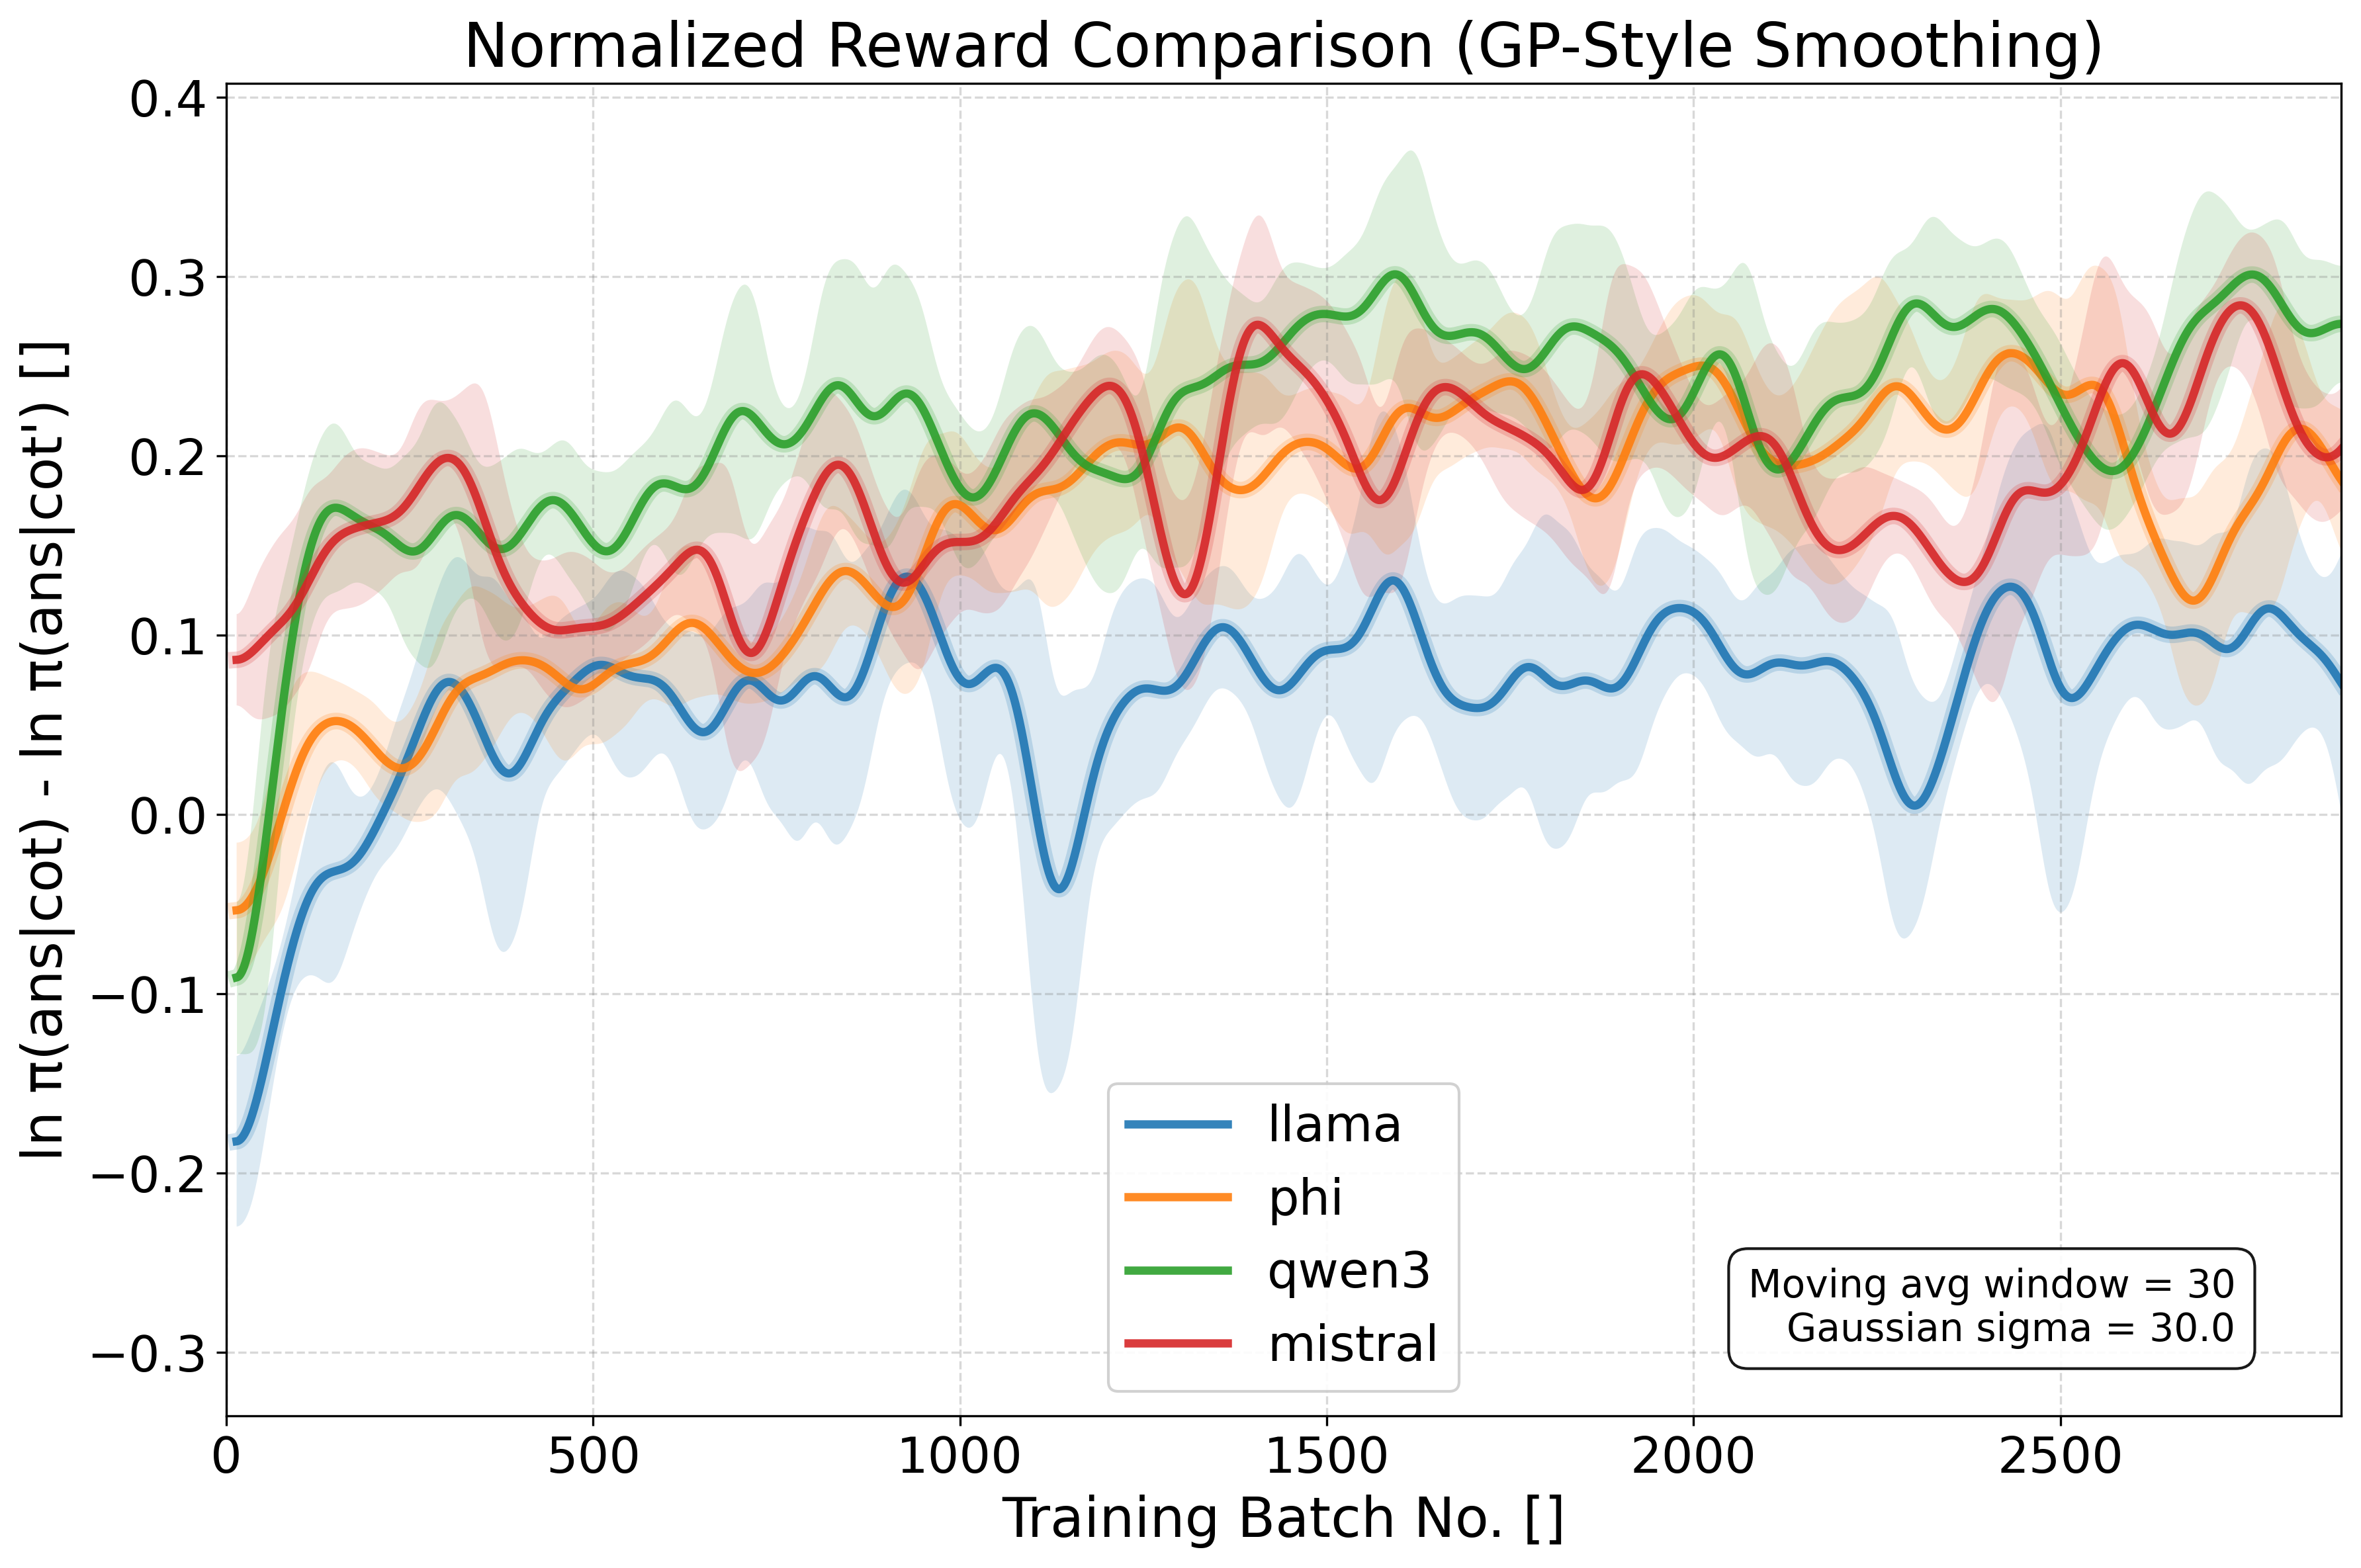
\includegraphics[width=\textwidth]{combined_normalized_reward_gp_smoothed.png}
%\caption*{\small Cross-model normalized reward on Wikipedia (Llama, Phi, Qwen, Mistral).}
%\end{figure}
%\end{columns}
%
%\vspace{0.3cm}
%Markovian training works across architectures --- not specific to Llama.
%\end{frame}

% ============================================================
\begin{frame}{Why Not Steganography?}

\textbf{Concern}: could the model encode the answer steganographically in the CoT?

\bigskip
\textbf{Three defenses}:

\begin{enumerate}
    \item \textbf{KL penalty} ($\beta = 0.1$): penalizes deviation from the pretrained CoT distribution, making unnatural encodings costly
    \item \textbf{Bounded CoT length}: limits the channel capacity
    \item \textbf{Inductive biases of gradient descent}: natural-language reasoning is the easier solution to discover
\end{enumerate}

\bigskip
\textbf{Empirical confirmation}: cross-model transfer to GPT-2 (124M params).
\begin{itemize}
    \item GPT-2 cannot decode sophisticated steganography
    \item Yet it benefits from Llama's trained CoTs
    \item $\Rightarrow$ CoTs use natural language, not model-specific codes
\end{itemize}
\end{frame}

% ============================================================
\begin{frame}{Limitations}

\begin{itemize}
    \item \textbf{Informativeness $\neq$ full faithfulness}: the CoT is sufficient for the answer, but may not mirror the model's exact internal computation
    \item \textbf{Human studies}: current verification uses perturbation fragility and cross-model transfer; direct human evaluation of CoTs is future work
    \item \textbf{Scaling}: tested up to 8B--12B parameters; larger models may behave differently
    \item \textbf{Post-hoc CoTs}: the model could compute the answer during question-reading passes and then generate a correct-but-post-hoc CoT (KL penalty + bounded length make this unlikely)
\end{itemize}

%\bigskip
%\textbf{Future work}:
%\begin{itemize}
%    \item Extend to multi-turn dialogue and longer reasoning chains
%    \item Human evaluation studies
%    \item Application to eliciting latent knowledge (ELK)
%\end{itemize}
\end{frame}

% ============================================================
\begin{frame}{Summary}

\begin{enumerate}
    \item \textbf{Markovian framework}: structural constraint forcing CoT to be causally essential (answer predicted from CoT alone)

    \item \textbf{GRPO-style training}: parallel sampling + actor-reward gradients + KL regularization through discrete text bottleneck

    \item \textbf{Strong performance}: large gains over base (GSM8K: 19.6\% $\to$ 57.1\%, ARC: 36.1\% $\to$ 79.9\%), competitive with Non-Markovian

    \item \textbf{CoTs are load-bearing}: perturbation analysis shows systematically higher sensitivity for Markovian models

    \item \textbf{CoTs are interpretable}: cross-model transfer (including to GPT-2) confirms natural-language reasoning
\end{enumerate}

\vspace{0.3cm}
\begin{center}
\Large Thank you!

\normalsize
Code: \texttt{github.com/scottviteri/MarkovianTraining}
\end{center}
\end{frame}

\end{document}
